\documentclass[a4paper,12pt]{report}
\usepackage[dvips]{color}
\usepackage{lscape}
\usepackage{color}
\usepackage{url}
\usepackage{rotating}
\usepackage[pdfborder={0 0 0}]{hyperref}
\usepackage{parskip}
\usepackage[margin=2cm]{geometry}
\usepackage[margin=2cm]{caption}
\usepackage{etoolbox}
\usepackage{longtable}
\usepackage{nicefrac}
\patchcmd{\quote}{\rightmargin}{\leftmargin 1em \rightmargin}{}{}

\usepackage{ulem}   % added by dave to allow strike-out below
\newcommand{\QUERY}[1]{{\color{red}{#1}}}
\newcommand{\NEW}[1]{{\color{blue}{#1}}}
\newcommand{\DEL}[1]{{\color{red}{\sout{#1}}}}
\newcommand{\COMMENT}[1]{{\color{magenta}{#1}}}

\usepackage{fancyhdr}
\usepackage{times}
\setlength{\headheight}{15pt}
 
\pagestyle{fancyplain}
\renewcommand{\chaptermark}[1]{\markboth{#1}{}}
 
\lhead{\fancyplain{}{\thepage}}
\chead{}
\rhead{\fancyplain{}{\textit{\leftmark}}}
\lfoot{}
\cfoot{}
\rfoot{}



%\hypersetup{
%    pdfborder={0 0 0}    % fits the width of the page to the window
%}


%\usepackage[Sonny]{fncychap}
%\usepackage[Bjarne]{fncychap}
%\usepackage[Lenny]{fncychap}
%\usepackage[Glenn]{fncychap}
%\newcommand{\ug}{$\mu g m^{-3}$}
%ST
\newcommand{\degrees}{\ensuremath{^\circ}}
 \newcommand{\ug}{\ensuremath{\mu \mbox{g m}^{-3}}\,}
\newcommand{\tug}{$\nicefrac{\mu g}{m^{3}}$}
\newcommand{\ugN}{\ensuremath{\mu \mbox{g(N) m}^{-3}}}
\newcommand{\tugN}{$\nicefrac{\mu g(N)}{ m^{3}}$}
\newcommand{\ugS}{\ensuremath{\mu \mbox{g(S) m}^{-3}}} 
\newcommand{\tugS}{$\nicefrac{\mu g(S)}{m^{-3}}$}

\newcommand{\mgSl}{\ensuremath{\mbox{mg(S)l}^{-1}}} 
\newcommand{\tmgSl}{$\nicefrac{mg(S)}{l}$} 
\newcommand{\mgNl}{\ensuremath{\mbox{mg(N)l}^{-1}}}
\newcommand{\tmgNl}{$\nicefrac{mg(N)}{l}$} 
\newcommand{\mgl}{\ensuremath{\mbox{mg l}^{-1}}}
\newcommand{\tmgl}{$\nicefrac{mg}{l}$} 
\newcommand{\mgSm}{\ensuremath{\mbox{mg(S)m}^{-2}}}  
\newcommand{\tmgSm}{$\nicefrac{mg(S)}{m^{2}}$} 
\newcommand{\mgNm}{\ensuremath{\mbox{mg(N)m}^{-2}}}
\newcommand{\tmgNm}{$\nicefrac{mg(N)}{m^{2}}$} 

%%% I tried using \bv to start a small-tex verbatim section and
%%% \ev to end this. However, it seems that \end{verbatim} needs to
%%% to be writtehn explcitly, so I use \ev now to end the small-text.
%%% Place directly after \end{verbatim}.

%% \newcommand{\bv}{\begin{small}\begin{verbatim}}
%% \newcommand{\ev}{\end{small}}

\newcommand{\Par}{{\bf Par\_ml}}
\newcommand{\MyOutputs}{{\bf My\_Outputs\_ml}}

\begin{document}
%\begin{landscape}

\title{The EMEP/MSC-W Model - User's Guide}
\date{October 2015}
\maketitle

\tableofcontents
\setcounter{page}{0}

\chapter{Welcome to EMEP }

This guide gives a brief documentation of the EMEP/MSC-W model
version rv4.8. 
It is intended primarily as a guide on how to run the model, and
to help users wishing to understand or change 
the model in terms of domains, outputs, chemistry, etc.


The main documentation for the EMEP/MSC-W model is an article pulished 
in Atmospheric Chemistry and Physics in 2012. 
This article will be referred to as Simpson et al. (2012) in
this manual. 


\begin{itemize}
\item
Simpson, D., Benedictow, A., Berge, H., Bergstr\"om, R., Emberson, L.D., Fagerli, H., Flechard, C.R., Hayman, G.D., Gauss, M., Jonson, J.E., Jenkin, M.W., Ny\'iri, \'A, Richter, C., Semeena, V.S, Tsyro, S., Tuovinen, J.-P., Valdebenito, \'A., and Wind, P.:
The EMEP MSC-W chemical transport model – technical description.  
Atmospheric Chemistry and Physics, 12, 7825-7865, 2012.\\
\url{http://www.atmos-chem-phys.net/12/7825/2012/acp-12-7825-2012.html}
\end{itemize}


The model source code is available from the EMEP/MSC-W Open Source website:\\ 
\url{https://wiki.met.no/emep/page1/emepmscw_opensource}

\newpage

\section{Licenses and Caveats}

The EMEP code is provided under the GNU General Public License version 3
(\url{http://fsf.org} and/or
\url{http://www.gnu.org/copyleft/gpl.html}).

Each code module is prefaced with something like:
\begin{quote}
\begin{small}
\begin{verbatim}
! <EXAMPLE_CODE.f90 - A component of the EMEP MSC-W  Eulerian
!          Chemical transport Model>
!*****************************************************************************!
!*
!*  Copyright (C) 2007-2012 met.no
!*
!*  Contact information:
!*  Norwegian Meteorological Institute
!*  Box 43 Blindern
!*  0313 OSLO
!*  NORWAY
!*  email: emep.mscw@met.no
!*
!*    This program is free software: you can redistribute it and/or modify
!*    it under the terms of the GNU General Public License as published by
!*    the Free Software Foundation, either version 3 of the License, or
!*    (at your option) any later version.
!*
!*    This program is distributed in the hope that it will be useful,
!*    but WITHOUT ANY WARRANTY; without even the implied warranty of
!*    MERCHANTABILITY or FITNESS FOR A PARTICULAR PURPOSE.  See the
!*    GNU General Public License for more details.
!*
!*    You should have received a copy of the GNU General Public License
!*    along with this program.  If not, see <http://www.gnu.org/licenses/>.
!*****************************************************************************!
\end{verbatim}
\end{small}
\end{quote}
And a copy of the license file, {\bf gpl.txt}, is provided with the
model code source files.

\noindent It is important to note that the code is provided ``as it is'', 
and EMEP/MSC-W has very limited resources with which to support
code-usage. 

%% To help users an {\bf EMEP Forum} is available from the
%% EMEP/MSC-W Open Source website in section ``Users'': ``EMEP Forum''. 
%% Support to the user community will develop here with your contribution. 
%% Please let us know what your needs for information are 
%% (e-mail: emep.mscw@met.no).

\newpage

\section{Computer Information}
\label{sec:compinf}

To compile the EMEP/MSC-W model you need:\\

\textbf{Fortran 95 compiler}

\textbf{NetCDF Library ($>$4.1.3)}

\textbf{MPI Library ($>$1.0)}\\

It is necessary to compile with double precision reals (8 bytes
reals). The program has been used on computers ranging from a Linux laptop to supercomputers 
(Itanium2 cluster, Intel Xeon cluster, Cray XT4, IBM power5+). It is compatible with all 
compilers tested so far:  Intel, PGI, gfortran, XL fortran. A Makefile is included,  
the path to netcdf (INCL and LLIB) have to be adapted to your machine, and the fortran 
compiler (F90) and flags (F90FLAGS) to the compiler you are using.



The code has been tested with 1 to 1024 CPUs, and scales well (for large grids).  If only one 
CPU is used 1-2 GB memory is required. If more than one,
for example 64 CPUs are used, 200 MB of memory per CPU is enough (in
the case of a 132 X 159 grid size). For runs on more than 32 CPUs, a fast interconnect is 
recommended (infiniband for example), for smaller runs, gigabit ethernet is sufficient. 
It takes $\sim$ 5 hrs on 64*Xeon X5355 (2.66GHz) for 1 year simulation.

When downloading input data in order to do a ``base run'' please make
sure that there are 35 Gb disc space available, especially due to
large meteorology input files. The model can be run for shorter periods, users 
can download meteorology for only the period they are interested in, pluss one day. 
 

\section{Getting Started}


It is recommended to read all the chapters of this EMEP/MSC-W model
User Guide before you start downloading anything from the EMEP/MSC-W Open
Source website.

%% Please register as an EMEP User on the {\bf EMEP Forum}
%% (EMEP/MSC-W Open Source website under ``Users'' section: ``EMEP Forum'')
%% before you start downloading the EMEP/MSC-W model code and/or input
%% data. This will give you access to further communication with the
%% developing team and to the section on ``Questions and Answers''. 


This is what you need to do before you can do a ``base run'' with the 
EMEP/MSC-W model:

\begin{itemize}
%\item Register as an EMEP User
\item Read the EMEP/MSC-W model User Guide
\item
Download input data (description in Chapter~\ref{ch:InputFiles} and
data available from the EMEP/MSC-W Open Source website under ``Download''
section: ``Input Data'')
\item
Download the EMEP/MSC-W model source code (description in 
section~\ref{sec:ModelCode} and the files are available from the EMEP/MSC-W 
Open Source website under ``Download'' section: ``Model Code'')
\item
Follow the instructions for 'Submitting a Run' description in
Chapter~\ref{ch:SubmitARun}.
\item
Download some model results for comparison, description in
Chapter~\ref{ch:output} and the files are available from the EMEP/MSC-W 
Open Source website under ``Download'' section: ``Model Results''. 
%NEWTOOLS:
% \item
% If wanted, download some helper programmes to read site and sonde outputs, 
% see sections~\ref{sec:tools},\ref{sec:sitesonde}.
% The files are available from the EMEP
% Open Source website under ``Download'' section: ``Tools''.


\end{itemize}

\section{Model code}
\label{sec:ModelCode}

The EMEP/MSC-W model code version rv.4.8 are archived as a tar file. 
The tar file is called ``EMEP\_MSC-W\_model.rv4.8.OpenSource.tar.gz'' and 
is downloadable from the EMEP/MSC-W Open Source website.

Once this file is untarred all model files needed for a model run will be 
found under the directory \\ {\bf EMEP\_MSC-W\_model.rv4.8.OpenSource/code/} 
where the model source code, makefiles, and a copy of the license file are 
stored. An overview is given in Table~\ref{Tab:modelfiles}

\begin{table}[h]
\begin{center}
\caption{Contents of ``EMEP\_MSC-W\_model.rv4.8.OpenSource.tar'' file
   \label{Tab:modelfiles}}
\begin{tabular}{ll}
& \\
\hline
Type      & Filename          \\
\hline
& \\
{\bf Model code directory} & EMEP\_MSC-W\_model.rv4.8.OpenSource/code \\ 
\hline
modules files & *.f90 \\
include files & *.inc \\
namelist & config\_emep.nml \\
makefiles & Makefile and Makefile.SRCS \\
dependency file &  dependencies\\
a copy of the license & gpl.txt \\
\hline
\end{tabular}
\end{center}
\end{table}

In addition there is a run script called ``modrun.sh'', which will be placed 
in the \\{\bf EMEP\_MSC-W\_model.rv4.8.OpenSource/}  directory. The run 
script, ``modrun.sh'', can easily be modified to work on your computer system. 
This script is described in detail in Chapter \ref{ch:SubmitARun}. 
 
%NEWTOOLS
% \section{Helper tools}
% \label{sec:tools}
% ????
% For users interested in reading the ascii site and sonde specific outputs,
% two help programmes (Rd\_sites.f90, Rd\_sondes.f90) are provided, 
% in the \\{\bf EMEP\_Unified\_model.OpenSource2012/tools}  directory. These
% programmes are readily compiled with e.g. gfortran, and can be run without
% arguments to obtain usage instructions. See section~\ref{sec:sitesonde}
% for more details.


\section{Model grid}
\label{sec:ModelGrid}

The current EMEP model version, and the provided gridded input data,
have a horizontal resolution of 50$\times$50 km$^2$ (at 60$^\circ$N)
and are defined on a
polar stereographic projection with 20 sigma levels vertically. 
The model is very flexible with regard to the horizontal
resolution, in that it readily makes use of 
meteorological data provided with the model. The vertical
resolution is currently still restricted to the fixed 20 layer
system. The physical
description is given in detail in Chapter 2 of the EMEP Status Report
1/2003 Part I (Simpson {\sl et al.}, 2003).

In 2008 the official EMEP domain was extended eastwards in order to include the 
EECCA countries in the EMEP model grid, see Figure \ref{fig:EECCA}. To distinguish the new grid from the old EMEP 
grid, the new grid is called EECCA in this text and in the config\_emep.nml.

\begin{figure}[ht]
 \centering
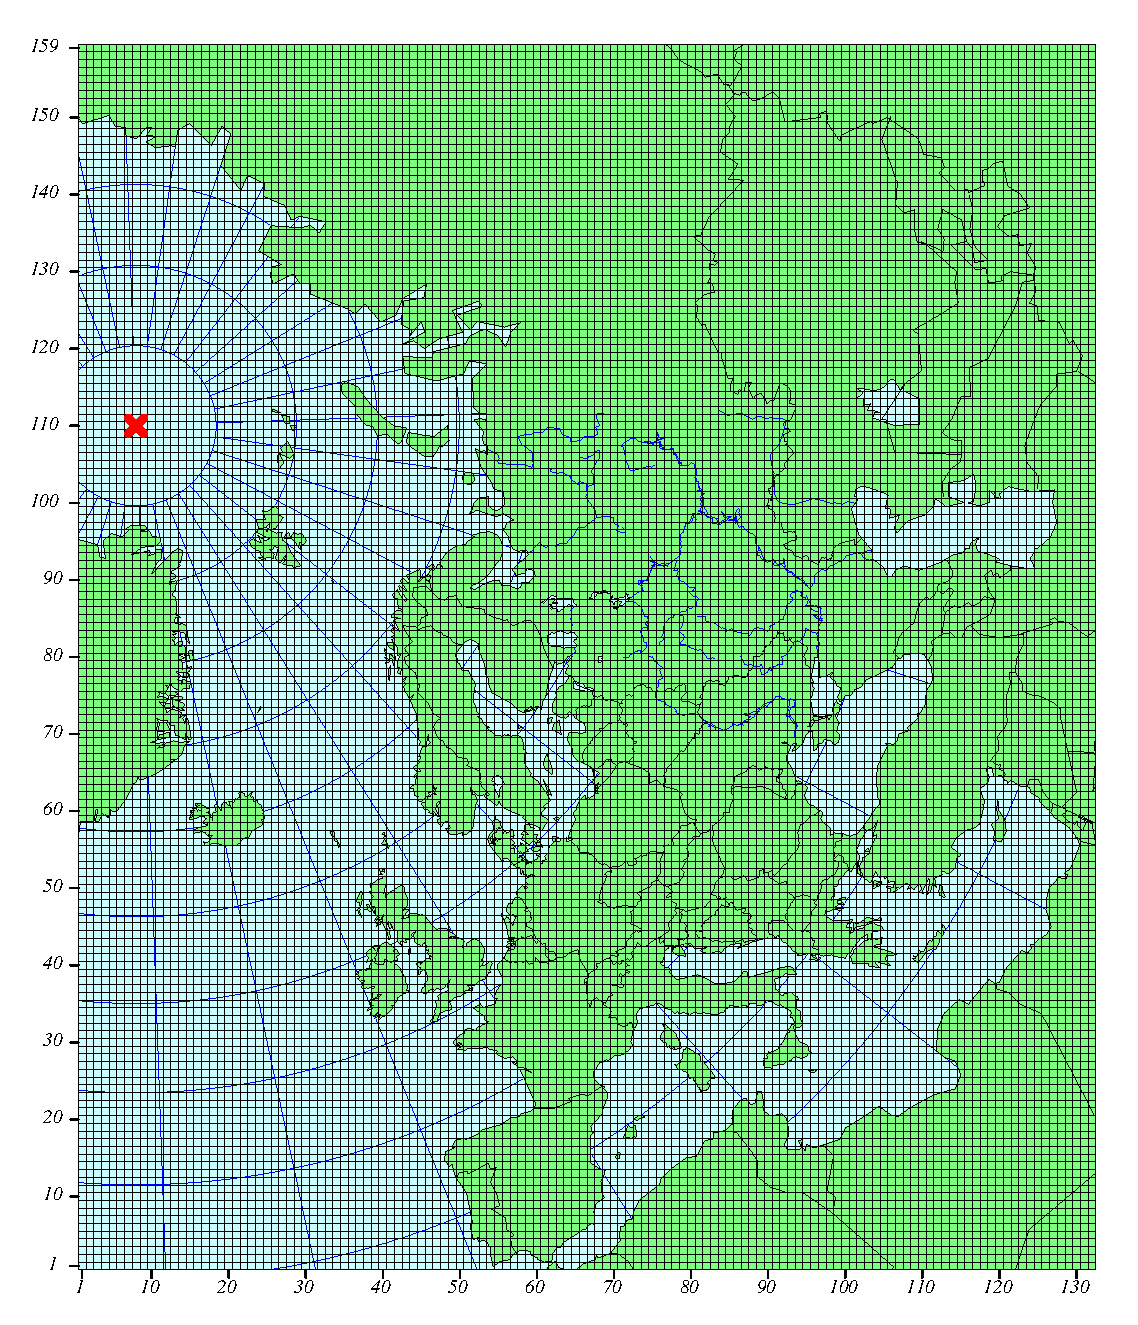
\includegraphics[scale=0.7]{EECCA.eps}
\caption{The extended EMEP grid covering EECCA area with
132$\times$159 gridpoints on 50$\times$50 km$^2$ resolution defined on a polarstereographic
projection.}\label{fig:EECCA}
\end{figure}



\chapter{Input files}
\label{ch:InputFiles}

This chapter provides an overview on the necessary input files to run 
the Unified EMEP model. A complete set of input files is provided in
the EMEP Open Source web page to allow model runs for the year 2005.

{\bf IMPORTANT:} The input data available in the EMEP Open Source Web
site should be appropriately acknowledged when used for model runs.
If nothing else is specified according to references further in this
chapter, please acknowledge EMEP/MSC-W in
any use of these data.

%%litt om filer og grid

%%asci vs netcdf

%tabell


\begin{table}
\caption[List of input data files]{List of input data files.
Note: YYYY: year, MM: month, DD: day, SEASON: seasons, POLL: pollutant
type (NH$_3$, CO, NO$_x$, SO$_x$, NMVOC,
PM$_{2.5}$ and PM$_{co}$). ASCII$^*$ means ASCII files with header.
\label{Tab:inputdata}}
\begin{small}
\hspace{-1cm}
\begin{tabular}{lll}
 && \\
\hline
{\bf Data} &  {\bf Name} & {\bf Format}\\
\hline\hline
% && \\
% {\bf Meteorology data directory} & EMEP\_metdata/YYYY/&  \\
\hline
Meteorology  &  meteoYYYYMMDD.nc \quad (366+1 files) & netCDF\\
& & \\
Boundary and initial conditions & Boundary\_and\_Initial\_Conditions.nc & netCDF\\
Landuse & Inputs.Landuse & ASCII$^*$\\
%BVOC emissions & Inputs.BVOC & ASCII$^*$\\
Land/Sea mask & landsea\_mask.dat & ASCII\\
Sites locations for surface output & sites.dat & ASCII$^*$\\
Sondes locations for vertical output & sondes.dat & ASCII$^*$\\
%Snow cover & snowcMM.dat.170  \quad (12 files) & ASCII\\
Natural SO$_2$ & natso2MM.dat  \quad (12 files) & ASCII\\
Volcanoes & Volcanoes.dat & ASCII$^*$\\
&& \\
{\bf Emission data directory } & EMEP\_GriddedData/Emissions/&  \\
\hline
Emissions & GridPOLL  \quad (7 files) & ASCII\\
&& \\
{\bf Grid-independent data directory} & Common/ & \\
\hline
Time factors for monthly emissions& MonthlyFac.POLL  \quad (7 files) & ASCII\\
Time factors for daily emissions &  DailyFac.POLL  \quad (7 files)
& ASCII\\
Landuse definitions & Inputs\_LandDefs.csv & ASCII$^*$\\
Stomatal conductance & Inputs\_DO3SE.csv & ASCII$^*$\\
Lightning emissions & lt21-nox.datMM  \quad (12 files) & ASCII$^*$\\
%Military aircraft emissions & amilt42-nox.dat & ASCII\\
%Commercial aircraft emissions & aSEASONt42-nox.dat \quad (4 files)& ASCII\\
Aircraft emissions & AircraftEmis\_FL.nc & netCDF \\
VOC speciation & vocsplit.defaults.BASE\_MAR2004 & ASCII\\
 & vocsplit.special.BASE\_MAR2004  & ASCII\\
NOx speciation & noxsplit.default.2000 & ASCII\\
 &noxsplit.special.BASE\_MAR2004& ASCII\\  
Emission factors for scenario runs & femis.dat & ASCII\\
Photo-dissociation rates & jclear.SEASON \quad (4 files) & ASCII\\
 & jcl1.SEASON \quad (4 files) & ASCII\\
 & jcl3.SEASON \quad (4 files) & ASCII\\
\hline
\end{tabular}
\end{small}


\end{table}

\subsection{NetCDF files}


The 3-hourly meteorological input data and the boundary and initial 
conditions input files are provided in netCDF format. 
We presently follow as much as possible the netCDF CF1.0 conventions 
(\url{http://www.unidata.ucar.edu/software/netcdf/}) for both input
and output data (except the Boundary\_and\_Initial\_Conditions file which
is still in GDV convention).

\subsubsection{Meteorology}

The meteorology input data is from the Integrated Forecast System (IFS), an global operational 
forecasting model from the European Centre for Medium-Range Weather Forecasts (ECMWF). 

The daily ``meteoYYYYMMDD.nc'' files with 3-hourly values are in netCDF 
(CF1.0 convention) format.

The parameters extracted from the ECMWF Meteorological output
currently used for Unified EMEP Model runs are given in 
Table~\ref{Tab:metinput}. A further description of these
meteorological fields is given in Chapter 3 of the EMEP Status Report
1/2003 Part I (Simpson {\sl et al.}, 2003).

{\bf Acknowledgement:} met.no

Please acknowledge The Norwegian Meteorological Institute in all
publications using these data.
 
\begin{table}[hb]
\caption{Input meteorological data used in the Unified EMEP Model
   \label{Tab:metinput}}
\begin{tabular}{p{6cm}lll}
\hline
Parameter      & Unit & Description          \\
\hline
\multicolumn{3}{l}{3D fields - for 20 $\sigma$ levels} \\
$u,v$  &  m/s     & Wind velocity components   \\
$q$    &  kg/kg   & Specific humidity           \\
$\dot{\sigma}$ & s$^{-1}$ & Vertical wind in $\sigma$ coordinates \\
$\theta$       & K  & Potential temperature \\
$CL$             & \% & 3D Cloud cover            \\
$PR$             & mm & Precipitation         \\
\hline
\multicolumn{3}{l}{2D fields - for Surface} \\
$P_s$             & hPa & Surface pressure                     \\
$T_2$          & K  & Temperature at 2m height               \\
$Rh_2$             & \% & Relative humidity at 2m height \\
SH              & W m$^{-2}$ & Surface flux of sensible heat \\
LH             & W m$^{-2}$ & Surface flux of latent heat \\
$\tau$         & M m$^{-2}$ & Surface stress               \\
SST            & K & Sea surface temperature \\
sdepth         & m & Snow depth \\
ice            & \% & Fraction of ice \\  
\hline
\end{tabular}
\end{table}

\subsubsection{Boundary and Initial Conditions}

Monthly files

D3\_O3\_Logan, D3\_CH3COO2,D3\_H2O2,D3\_OH

\subsection{Landuse}

Landuse data are required for modelling booundary layer processes
(i.e. dry depositon, turbulent diffusion).
The Unified EMEP model can accept landuse data from any
data set covering the whole of the domain and providing reasonable 
resolution of vegetation categories. Gridded data sets providing
these landuse categories across the EMEP domain have been created
based on the data from the Stockholm Environment Institute at York 
(SEI-Y) and from the Coordinating Centre for Effects (CCE). 
16 basic landuse classes have been identified for use in the
deposition module in the model, and three additional``fake'' landuse
classes are used for providing results for integrated assessment
modelling and effects work.

There is a {\bf header} in the file that contains short abbreviations 
for the different landcover
types, e.g. CF for temperate/boreal coniferous forest. The landuse
types are summarised in Table 5.1 in Chapter 5 of the EMEP Status
Report 1/2003 Part I (Simpson {\sl et al.}, 2003).

The different landuse types are given as a percentage of area for each 
EMEP grid cell in the {\bf ASCII file} ``Inputs.Landuse''. 



\subsection{Land/Sea mask}
This file, based on HIRLAM roughness length is used
to assign land/sea mask within the Unified EMEP model, since there is
a need to modify the stability information for coastal grid cells
(which contain land, but is not resolved by the NWP model supplying 
meteorological data to the Unified EMEP model). 

The gridded {\bf ASCII} file ``landsea\_mask.dat'' contains 3 columns. 
The first two columns represent the `i' and `j' indices of the EECCA
grid and the third column gives the class of the grid cell, where the 
EMEP model use 0 for ocean, and $\geq$ 1 as land.% length with unit: $m$.

\subsection{Site and Sonde locations for output}\label{sec:sitessondes_input}
The model provides a possibility for extra output data of surface concentration 
for a set of specified measurement site locations and concentrations for the vertical 
column above a set of specified locations. These site and sonde locations are listed 
in the {\bf ASCII} files ``sites.dat`` and ``sondes.dat`` files. These files can be 
changed by the user, this is described in section \ref{sec:sitesonde}.


\subsection{Natural $SO_2$}
Natural $SO_2 emissions$ (dimenthylsulfide (DMS) from sea) are provided 
an monthly gridded files. They are stored in columns of `i' and `j' and the 12 monthly `values'. 
The values are given at the surface in $\mu g /m³ $ for each grid cell in the domain. 

\subsection{Volcanoes}

Emissions of volcanoes are included for Italy, based upon the
officially submitted data.
To consider the volcanic emissions, we need to feed the location
and height of volcanoes into the model. 

The input file ``Volcanoes.dat'' in {\bf ASCII} format contains the input data for the two active volcanoes
 Enta and Stromboli. The two first colums gives their latitudes and longitudes, their height as sigma level
 in column 3 and their emission in ktons per year in column 4. 

\subsection{Emissions}
The emission input for the Unified EMEP model consists of gridded
annual national emissions based on emission data reported every year
to EMEP/MSC-W (until 2005) 
and to CEIP (from 2006) by each
participating country. 
More details about the emission input with references can be
found in Chapter 4 of the EMEP Status Report 1/2003 Part I 
(Simpson et al., 2003).

The 7 gridded emission input files ``gridPOLL'' are available in 
{\bf ASCII} format for the following compounds: CO, NH$_{3}$,
NO$_{x}$, PM$_{2.5}$, PM$_{co}$, SO$_{x}$ and VOC.

The gridded emission files contain 16 columns where the first column 
represents the country code
(\url{http://www.emep.int/grid/country_numbers.txt}), 
the second and the third columns are the `i' and `j' indices of the
EMEP grid, the fourth and fifth columns are the total emissions from
low and high sources, and the rest 11 columns contain emissions from 
10 anthropogenic SNAP sectors 
(\url{http://reports.eea.eu.int/technical_report_2001_3/en}) and 1 
source-sector called``Other sources and sinks'', which include natural and
biogenic emission sources. The data are given with the unit: $Tonnes$.

{\bf Acknowledgement:} EMEP

\subsection{Time factors for emissions}

Monthly and daily time factors for emission of the 7 compounds 
(CO, NH$_{3}$, NO$_{x}$, PM$_{2.5}$, PM$_{co}$, SO$_{x}$ and VOC). 
There is one file available per compound in {\bf ASCII} format. 

The first two columns in the files represent the country code
(\url{http://www.emep.int/grid/country_numbers.txt}), the second column 
represents the sector (\url{http://webdab.emep.int/sectors.html}. In the monthly files, 
the 12 consecutive columns represent the time factors corresponding to 
the months of the year. In the daily files there are 7 consecutive columns representing 
the time factor for each day of the week. 

\subsection{Landuse definitions}
For those vegetative landuse categories for which stomatal modelling is
undertaken, the start and end of the growing season (SGS, EGS) with
latitude dependent data to capture north-south differences and the
development of the leaf area index (LAI) within this growing season
must be specified. There is a schematic of LAI development in Figure
5.1 in Chapter 5 of the EMEP Status Report 1/2003 Part I (Simpson {\sl et al.}, 2003).

The {\bf ASCII} file ``Inputs\_LandDefs.csv'' provides land-phenology data
of each landuse type summarised in Table 5.1 in Chapter 5 of the EMEP 
Status Report 1/2003 Part I (Simpson {\sl et al.}, 2003) for dry deposition 
calculations.

The file contain a {\bf header} explaing briefly the contents of the 
14 columns. 
The first three columns are representing the landuse name, code (which
are consistent with those in ``Landuse.Input'' file) and
type (grouping of the landuse classes). The fourth column gives
the maximum height of vegetation ($m$), the fifth indicates albedo (\%) and
the sixth indicates possible source of NH$_{x}$ (0/1). 7 to 10
column is about growing season (day number), 11 and 12 indicates the
LAI minimum  and maximum ($m^{2}/m^{2}$) and then 13 and 14 column
represent the length of the LAI increase and decline periods (no. of days).


\subsection{Stomatal conductance}
Parameters for the stomatal conductance model, deposition of O$_{3}$ and
stomatal exchange (DO3SE) that are based upon the ideas in
Emberson {\sl et al.}, 2000, and further discussed in Simpson and Emberson,
2006, must be specified.  

The {\bf ASCII} file ``Inputs\_DO3SE.csv'' provides land-phenology data
of each landuse type summarised in Table 5.1 in Chapter 5 of the EMEP 
Status Report 1/2003 Part I (Simpson {\sl et al.}, 2003) for stomatal
conductance calculations.

The file contains a {\bf header} indicating the contents of the file
with the different factors needed for each of the landuse classes used
in the Unified EMEP model. The first two columns are representing the
landuse code (which are consistent with those in ``Landuse.Input'' file)
and name. The next 22 values are different phenology factors.

\subsection{Lightning emissions}
Emissions of NO$_{x}$ from lightning are included in the model
as monthly averages on a T21 (5.65$^{\circ}$$\times$5.65$^{\circ}$) resolution (K{\o}hler {\sl et al.}, 1995). 
The lightning emissions are defined on a 64$\times$32 grid with 17 vertical
levels, with global coverage and are provided as 12 {\bf ASCII} files
``lt21-nox.datMM''.


\subsection{Aircraft emissions}
In the Unified EMEP model aircraft emissions are 'OFF' by default. 
They can be switched 'ON' by setting USE\_AIRCRAFT\_EMIS = TRUE in ModelConstants\_ml.f90. 
The model will then use data provided by the EU-Framework Programme 6 Integrated 
Project QUANTIFY (\url{http://www.pa.op.dlr.de/quantify}). However, before using 
these data a protocol has to be signed, which is why the data file can not be provided 
directly on the EMEP Open Source website. If you want to use aircraft emissions go to 
\url{http://www.pa.op.dlr.de/quantify}, click on 'QUANTIFY emission inventories and scenarios', 
and then click on 'Register'. That page will provide information about the registration 
process and the protocol that has to be signed. Once you are registered, click 'Login' and 
provide username and password. On the new page, search for 'Emissions for EMEP', which 
links directly to the Readme file and the emission data file on netCDF format. Download the 
emission data file and place it in the input folder.

\subsection{VOC speciation}
Speciation of VOC emissions are specified for each source-sector,
derived from the detailed United Kingdom speciation given in PORG
(1993). The Unified EMEP model uses a `lumped-molecule' approach to
VOC emissions and modelling, in which for example model species NC4H10
represents all C3+ alkanes, and o-xylene represents all aromatic
species. Therefore, each of the species from the detailed UK inventory
has been assigned to one of the Unified EMEP model's species according
to its reactivity and chemical composition, as given in
Andersson-Sk\"{o}ld and Simpson (1997). Although the exact VOC speciation
used can be varied (``vocsplit.special.BASE\_MAR2004'') to suit
particular emission scenarios (e.g. Reis {\sl et al.}, 2000), a default split
(``vocsplit.defaults.BASE\_MAR2004'') is typically used, as given in
Table 4.3 in Chapter 4 of the EMEP Status Report 1/2003 Part I (Simpson {\sl et al.}, 2003).

There are two available {\bf ASCII} files which one can choose to
run the model with, depending on whether a particular scenario should be
suited or not. However, the files
``vocsplit.defaults.BASE\_MAR2004'' and ``vocsplit.special.BASE\_MAR2004''
have currently the same content.

\subsection{NOx speciation}
Speciation of NO$_x$ emissions are specified for each source-sector and
for each country if the file ``noxsplit.special.BASE\_MAR2004'' is
chosen for the model run. The amount of NO$_{2}$ compared to
other NO is determined by these split-files.

There are two downloadable {\bf ASCII} files which one can choose to
run the model with, depending on whether a particular scenario should be
suited or not.
The file ``noxsplit.default.2000'' is only sector dependent and the file
``noxsplit.special.BASE\_MAR2004'' is both sector and country dependent.

\subsection{Emission factor for scenario runs}
Scenario run in the case of the Unified EMEP model means a run to test
the impact of one or more pollutants from a particular
country. 

Emission factors are applied to specified countries and
emission sectors and can be set by changing the {\bf ASCII} file
``femis.dat''. 
This file can be changed by the users according to their needs.

The file contains 10 columns. The first column represents
the country code (\url{http://www.emep.int/grid/country_numbers.txt}),
the second represents the sector
(\url{http://reports.eea.eu.int/technical_report_2001_3/en}) 
where `0' means all sectors, and then in the next 7 columns one can specify
which emissions to reduce. Here 1.0 means 100\% emissions of the given
pollutant 
(sox/nox/voc/nh3/co/pm25/pmco) from sectors of specified country. The
number following the first text (``Name'') in line 1 (number 5 in
the downloaded file) gives the number of pollutants treated in the file.

\subsection{Photo-dissociation rates}
The photo-dissociation rates (J-values) are provided as lookup
tables. The method is previously described in Jonson {\sl et
al.}, (2001). J-values are provided as clear sky, light cloud and dense
cloud conditions, and the model interpolates between these according
to cloudiness from the meteorological input data. In the lookup tables
data are listed for every 10 degree latitude at an interval of 1
degree zenith angle at every model height.

For the two types of cloud conditions there are one {\bf ASCII} file 
averaged for each season; January, April, July and October (jan represents
winter, apr represents spring, jul represents summer, oct represents
autumn). For light
cloud the four seasonal files are called ``jcl1.SEASON'', for dense cloud conditions
the four seasonal files are called ``jcl3.SEASON'', and then for clear sky the one file 
is called ``jclear.dat''.

Each file contains 18 columns. The first column is latitude of zenith 
angle and then the
next 17 are the values for the model levels with the unit: $1/s$. 
For more details about these rates, please read Chapter 7.2 of the EMEP
Status Report 1/2003 Part I (Simpson {\sl et al.}, 2003).


\chapter{Output files}
\label{ch:output}

Output files from a model run are written out in either ASCII, or
(for most data outputs) in netCDF format. 
The different netCDF files, the Runlog output, and the zipped sites and sondes 
files are named after the runlabel1 parameter set in modrun.sh. 
The model output is written to the same directory as where you submitted 
your run with the modrun.sh script, as described in Chapter \ref{ch:SubmitARun}.

To compare you you model results, there has been made available model result files 
that can be downloaded  from the EMEP Open Source website under ``Download'' section: ``Model Results''. 
There are both model results for a run over a whole year, and a test run over two days from 
January 1$^{st}$ to 2$^{nd}$. These are placed in an output/ directory. 
 

\begin{table}[h!]
\caption[List of model output files]{List of output files written in the
  working directory after a  model run. 
Note: YY: year, MM: month.}\label{tab:output}
% \vspace{0.5cm}
\begin{center}
\hspace{-1cm}
\begin{tabular}{lll}
\hline
{\bf Output data files} &  {\bf Short description} & {\bf Format}\\
\hline
    Base\_day.nc & Gridded daily values of a selection & netCDF\\
&   of compounds.& \\ 
    Base\_hour.nc &Gridded hourly values of a selection &
    netCDF\\  
 &  of compounds.& \\
%    Base\_inst.nc &Gridded instantaneous values of a selection
%     & netCDF\\
 &  of compounds.& \\
    Base\_month.nc & Gridded monthly values of a selection&
    netCDF\\
 &  of compounds.& \\
    Base\_fullrun.nc & Gridded yearly values of a selection&
    netCDF\\
 &  of compounds. & \\
    sites.MMYY & Surface daily values of a selection&  ASCII\\
 & of stations and compounds per month.& \\
%    Base.sites.tgz & All the 'sites.MMYY' files in one zipped tar file. & ASCII\\
    sondes.MMYY & Vertical daily values of a selection& ASCII\\
 &  of stations and compounds per month.& \\
%    Base.sondes.tgz& All the 'sondes.MMYY' files in one zipped tar file.& ASCII\\ 
& &\\ \hline
{\bf Additional files} &  {\bf Short description} & {\bf Format}\\
    Base\_RunLog & Summary log of runs, including total emissions  & ASCII\\
 &  of different air pollutants per country& \\
%% eulmod.res & Mass budget for different compounds & ASCII\\
% INPUT.PARA & List of input parameters & ASCII\\\hline
% Remove.sh & Removes the links to the input data at the& ASCII\\
% & end of the run&\\\hline
Timing.out & Timing log file& ASCII \\
 
\hline
\end{tabular}
\end{center}

\label{Tab:outputs}
\end{table}


\newpage
\section{ASCII outputs: sites and sondes}\label{sec:sitesonde}


Two main options are available for the output of ASCII files for comparison
with measurements or detailed model analysis. These are

\begin{description}
\item[sites]  

      output of surface concentrations for a set of specified
      measurement site locations.
\item[sondes] 

      output of concentrations for the vertical column above
     a set of specified locations.
\end{description}

Both sites and sondes are specified and handled in similar ways, in
the module {\bf Sites\_ml.f90}, so we treat them both together below.
Locations are specified in the input files ``sites.dat'' and ``sondes.dat''. 
The files start with a description of its content
followed by a list of the stations. For example, a sondes.dat input file
may look like this:

\begin{small}
\begin{quote}
\begin{verbatim}
# "Sondes: names, locations, elevations"
# "Area: Northern Hemisphere"
# "latitude in degrees (positive north)"
# "longitude in degrees (positive east of Greenwich)"
: Units deg
: Coords LatLong
: VertCoords EMEPsigma
: DomainName Hemis
#
name lat long lev #HEADERS
-    deg deg level #SKIP
#DATA:
Uccle             50.80    4.35  20  ! comment
Lerwick           60.13   -1.18  20  ! comment
Sodankyla         67.39   26.65  20  ! comment
Ny_Alesund        78.93   11.88  20  ! comment
Hohenpeissenberg  47.80   11.02  20  ! comment
\end{verbatim}

\end{quote}
\end{small}

Or, in cases where grid indicies are used rather than latitudes and 
longitudes. This is useful if you want sites and sonde output from a line 
or an area from the model. 

\begin{small}
\begin{quote}
\begin{verbatim}
# "Sites: names, locations, elevations"
# "Area: EMEP-EECCA"
# "ix: x coordinate"
# "iy: y coordinate"
# "lev: vertical coordinate (20=ground)"
: Units index
: Coords ModelCoords
: VertCoords EMEPsigma
: DomainName EMEP-50kmEECCA
#
name ix iy lev #HEADERS
-    index index level #SKIP
#DATA:
\end{verbatim}

\end{quote}
\end{small}

The first line in each file is a header with file content.
Then, the contents are described in more detail. Text strings after
\# are just clarifying comments. 'Area', e.g., is the domain to which
the stations belong, e.g. 'Northern Hemisphere'.

Text after ':' is read in by the model:\newline
- Units: either 'deg' (degrees) or 'index' (model grid indices)\newline
- Coords: either 'LatLong' (latitudes/longitudes) or 'ModelCoords'
(indices of the grid box in which the station is located)\newline
- VertCoords: vertical coordinate system that is used in the model (usually
'EMEPsigma')\newline
- DomainName: domain, for which the model is run (e.g. 'Global\_1x1' or 'Hemis')\newline


Both sites.dat and sondes.dat files are optional, but recommended. 
The species and meteorological data requested for site and sone output
 are specified in {\bf My\_Outputs.f90} by the use of arrays. Only a 
few met fields are defined so far but more can be added into 
{\bf Sites\_ml.f90} as required. 

The outputs consist of a header giving the number of sites requested, 
species/met data requested, and then the actual values for each 
variable for each staion. For the sonde data values are given for 
all 20 levels, starting with the ground-level values. These files
are best read using some helper programmes, which we provide in
the "Tools" directory:

\begin{description}
\item[Rd\_sites.f90] - reads the sites outout file for one month, and allows the
user to select site and component. Produces several outputs (SITES.hrly etc.), including
hourly values, daily mean and max. The code is quite short and easy to modify
\item[Rd\_sondes.f90] - similar to Rd\_sites, but for the sondes output.
\end{description}

Simply compile and run the executable to obtain usage instructions.


\newpage

\section{NetCDF outputs, Derived fields}

%{\bf modules My\_Derived\_ml, Derived\_ml }\\

% My\_Derived\_ml:\\
% \begin{itemize}
%   \item Constructs arrays wanted\_deriv2d, wanted\_deriv3d, listing
%    the outputs which the user wants in netcdf fields.
% \end{itemize}
% 
% Derived\_ml:\\
% \begin{itemize}
%   \item Contains definitions of possible output fields
%   \item Allocates data arrays d\_2d and d\_3d for those
%     fields which were requested in My\_Derived\_ml	
% \end{itemize}

The netCDF output files can contain both 2D and 3D data fields. The module 
{ \bf Derived\_ml.f90 } contains an extensive set of predefined outputs, and
others are defined as required in { \bf My\_Derived\_ml.f90}. 
The user may choose which of these possible data fields should be written 
into the output files by modifying the module called { \bf My\_Derived\_ml.f90}.\\

Most data fields are defined by the array OutputConcs. A defined output 
field for ozone in ppb is for example given  as:
\begin{quote}
\begin{verbatim}

 typ_s5i("O3        ", "ppb", D2,"AIR_CONCS", SPEC, D),& 

\end{verbatim}
\end{quote}
This will give a 'SURF\_ppb\_O3' 2-dimensional surface field in the output netCDF file for 
the fullrun, monthly and daily output. 
Setting the dimensions to D3 will give an additional 3-dimensional field. 


Other arrays where output fields are given are D2\_SR, D2\_EXTRA,\
 VEGO3\_WANTED and 
WDEP\_WANTED. Other fields are also defined in { \bf My\_Derived\_ml.f90 } e.g. for dry 
depositions, emissions, canopy etc. \\



Note that by default the maximum field of 2- and 3-dimensional output field are 
restricted to 200 and 5 respectively. These can be changed with MAX\_NUM\_DERIV2D and MAX\_NUM\_DERIV3D 
in { \bf My\_Derived\_ml.f90 }.


The output frequency is set in { \bf Derived\_ml.f90 }, for example for the surface fields:
\begin{quote}
\begin{verbatim}

 call AddNewDeriv( "PSURF ","PSURF",  "SURF","-",   "hPa", &
               -99,  -99,  F,  1.0,  T,   IOU_DAY )

\end{verbatim}
\end{quote}
 Where the IOU\_DAY setting gives the field in the fullrun.nc, month.nc in addition to the day.nc 
model output files. IOU\_MON gives the field in the fullrun.nc and the month.nc file. 




\chapter{Submitting a Run}
\label{ch:SubmitARun}

In this chapter we provide detailed information on how to run the
regional Unified EMEP model for two different types of
simulations, namely: 

\begin{itemize}

\item {\bf Base run} \\
This is the default set up for yearly transport model calculations
in 50x50 km$^2$ grid. 
\item{\bf Scenario run} \\
 A run with reduced emissions from a particular country or several
 countries is called 
a ``Scenario run''. It is the basic type of run for source-receptor
calculations. 

\end{itemize}

\noindent
Details about the submission of these
different types of runs are given below. We suggest that users test
the ``Base run'' first, which can be done without significant changes in
the code itself. One can also use the outputs of such a run in the
future as a reference run for the other simulations.\\  
% 
% As explained in the previous chapters, once the model tar file is
% untarred and all the files are located in the directory called
% {\sl Unify/Unimod.rv3\_7/}, one can find the run script with name
% ``modrun.sh'' in this 
% directory.

\newpage
\section{Base run}

This is an example of a minimum modrun.sh script to run the model.


\begin{verbatim}
#!/bin/bash

#Minimum script to run the emep model

#link to the input data
inputdir=./Base
ln -s $inputdir/* .

#define some input data
trendyear=2008 #emission year
runlabel1=rv3_7 #short label
runlabel2=Opensource_setup #long label
startyear=2008 #start year (metdata)
startmonth=1 #start month (metdata)
startday=1 #start day (metdata)
endmonth=1 #end month (metdata)
endday=31 #end day (metdata)

#put input data into a temporary file called INPUT.PARA
cat>>    'INPUT.PARA'<<    EOF
$trendyear
$runlabel1
$runlabel2
$startyear
$startmonth
$startday
$endmonth
$endday
EOF

#run the model
mpirun Unimod

#clean the links to the input data
ls $inputdir|xargs rm
rm INPUT.PARA

\end{verbatim}

The script is pretty self-explanatory, first the script links 
all the input files so you check if all the input files are in 
the right directory. 
The trendyear can be set to change the boundary emissions for 
earlier and future years, see the modules {\bf BoundaryConditions\_ml.f90 } 
and {\bf GlobalBCs\_ml.f90 } to understand better what the trendyear 
setting does. 
The runlabel1 option sets the name of the different output netCDF 
files. 
Startyear has to be set equal to the year 
that the metdata is available. The period you want to run the 
EMEP model is set with startmonth, and startday and the last day is 
set with endmonth and endday. \\

It is recommended to submit the script as a batch job. Please check the submission soutine 
on the computer system you are running on. 
When setting the number of nodes, it is important that it equals to the number set in the fortran module 
{\bf ModelConstants\_ml.f90}. In the module you set the wanted nodes in the x- and y-direction with NPROCX and 
NPROCY. The sum of these two is the number of nodes used. \\

When the job is no longer model is finnished or has crashed for some reason, there will be an output log file and 
an error file in the directory. If the run was successful, a message stating 
\begin{verbatim}
Eulmod: Successful exit atCET ..date..
\end{verbatim}
will be stated at the end of the log file, before listing up site and sonde files. 
The model results will also produced in the same directory, or you can set you own working directory in 
the script. For more information about the model results output files, see chapter \ref{ch:output}.\\

If for some reason 
the model crashed, please check both the log and error file for any clue of the crash. After fixing the 
problem the job can be submitted again. If the model has crashed, then the links to the inputdatas are not cleaned. 

The script can also be submitted interactivelly, and either have the output be written to the screen or to 
named output log and error files. 
 


\subsection{Setting the model domain}

It is possible to run the model on a smaller domain than the full
regional model domain, which is defined by  x coordinates ranging
from 1 to 132 and y coordinates ranging from 1 to 159. 

To set a smaller domain, one needs only to specify the
coordinates of the new domain in {\bf RUNDOMAIN} in the Fortran module
called {\bf ModelConstants\_ml.f90}. For example:


\begin{verbatim}
  
   !                    x0   x1  y0   y1
        RUNDOMAIN = (/  36, 100, 50, 150 /)  ! smaller EECCA domain

\end{verbatim}

tells the model to run in the domain with x coordinates ranging from
36 to 100 and y coordinates from 50 to 150.\\ 

\section{Scenario run}

The EMEP  model can be used to test the impact of reduced emission of
one or more pollutants from a particular country or a number of
countries.  Such runs are called ``Scenario runs''. They are the basic
runs for source-receptor calculations.


Emission factors for reduced emissions of pollutants from different
sectors and countries can be defined in the input file called
``femis.dat'', which can be found in the downloaded input data
directory, {\sl input\_data/Common/}.

An example of the ``femis.dat'' file for a base run is shown below:

\begin{verbatim}
------------------------------------------
Name  5     sox    nox   voc   nh3  pm25
27    0     1.0    1.0   1.0   1.0  1.0  

------------------------------------------
\end{verbatim}

\noindent
This base run example means that there is 100\% (1.0) emission of sox (SO$_x$),
nox (NO$_x$), voc (VOC), nh3 (NH$_3$) and pm25 (PM$_{2.5}$) from all
sectors in the UK. 

\begin{itemize}

\item The first column of
the second line represents the country code. (27 is the code for UK.)
The codes for all countries can be found in  Fortran module {\bf
  Country\_ml.f90}. Please note that the country code must be the same
which is used in the emission files for the given country. Some
countries and areas are divided into sub-areas in the emission
files. In this case, one line for each sub-area has to be included
into the ``femis.dat'' file. Countries and areas where emissions are
given for sub-areas include the Russian Federation, Germany and all 
sea areas.    

\item The second
column of the second line 
represents the sector and ``0'' means all sectors. Here one can write
the appropriate sector code if the emission is reduced only from a specific
sector. The description of each sector can also be found in the Fortran
module {\bf EmisDef\_ml.f90}. 

\item The columns under the pollutant names show the emission factors
  for the given pollutants. For example, 0.7 would mean 70\% of the
  original emission, thus 30\% reduction.


\item The number (``5'') following
the first text (``Name'') in the first line gives the number of
pollutants treated in the file.   
              
\end{itemize}

An example of ``femis.dat'' file describing 50\% reduced emission of
``sox'' from sector 10 (the emission from agriculture) in the UK can be given as:  

\begin{verbatim}
-----------------------------------------
Name  5    sox    nox   voc   nh3  pm25 
27    10   0.5    1.0   1.0   1.0  1.0   

-----------------------------------------
\end{verbatim}        

For a scenario run ``femis.dat'' file should be edited 
manually depending on the factor of
reduction one would like to test with any pollutant from any sector
and/or any country. Several lines can be written in the file.

Once the ``femis.dat''  file is
edited, the run can be submitted.  





\chapter*{References}
\label{ch:References}

\begin{description}

\item[Andersson-Sk{\"o}ld and Simpson, 1997] Y. Andersson-Sk\"{o}ld
  and D. Simpson. Comparison of the chemical schemes of the {EMEP MSC-W}
		  and the {IVL} photochemical trajectory models. EMEP
                  MSC-W Note 1/97. The Norwegian
Meteorological Institute, Oslo, Norway, 1997.

\item[Emberson {\sl et al.}, 2000] L. Emberson, D. Simpson,
  J.-P. Tuovinen, M.R. Ashmore and H.M. Cambridge. Towards a model of
  ozone deposition and stomatal uptake over Europe. EMEP/MSC-W
  Note 6/2000.

\item[Fagerli {\sl et al.}, 2004] H. Fagerli, D. Simpson and
  S. Tsyro.
 Unified EMEP model: Updates. In {\it EMEP Status Report
    1/2004, Transboundary acidification, eutrophication and ground
    level ozone in Europe. Status Report 1/2004}, pages 11--18. The Norwegian
Meteorological Institute, Oslo, Norway, 2004.

\item[Gardner {\sl et al.}, 1997] R.M. Gardner, K. Adams, T. Cook,
  F. Deidewig, S. Ernedal, R. Falk, E. Fleuti, E. Herms, C.E. Johnson,
  M. Lecht, D.S. Lee, M. Leech, D. Lister, B. Masse, M. Metcalfe,
  P. Newton, A. Schmitt, C. Vandenbergh and R. Van Drimmelen. The
  ANCAT/EC global inventory of NO$_x$ emissions from 
		  aircraft. {\it Atmos. Environ.}, 31 (12): 1751-1766
, 1997.


\item[Jonson {\sl et al.}, 2001] J.E.Jonson, J.K.Sundet and
  L. Tarras{\'o}n. Model calculations of present and future levels of
ozone and ozone precursors with a global and a regional model. {\it
  Atmos. Environ.}, 35: 525-537, 2001.  


\item[K{\"o}hler {\sl et al.}, 1995] I. K{\"o}hler, R. Sausen and
  G. Klenner. 
NO$_x$ production from lightning. The impact of NO$_x$ emissions from
aircraft upon the atmosphere at flight altitudes 8-15 km (AERONOX),
edited by U. Schumann, final report to the Commission of the European
Communities, Deutch Luft und Raumfart, Oberpfaffenhofen, Germany,
343--345, 1995.


\item[Logan, 1998] J. A. Logan. An analysis of ozonesonde data for the
  troposhere: Recommendations for testing 3-D models and development
  of a gridded climatology for troposheric ozone. {\it
    J. Geophys. Res.}, 10 (D13):16, 115--116, 149, 1998.


\item[Reis {\sl et al.}, 2000] S. Reis, D. Simpson, R. Friedrich,
  J.E. Jonson, S. Unger and A. Obermeier. Road traffic emissions -
  predictions of future  contributions to regional ozone levels in Europe.
{\it Atmos. Environ.}, 34: 4701-4710, 2000.

\item[Simpson {\sl et al.}, 2003] D. Simpson, H. Fagerli, J.E. Jonson, 
                    S. Tsyro, P. Wind and J.-P. Tuovinen.
{\it The EMEP Unified Eulerian Model. Model Description. EMEP MSC-W Report
1/2003}. The Norwegian
Meteorological Institute, Oslo, Norway, 2003.


\item[Simpson and Emberson, 2006] D. Simpson and L. Emberson. Ozone
  fluxes -- Updates.  
% L. Tarras{\'o}n,
%  H. Fagerli,  H. Klein, D. Simpson, A.C. Benedictow, V. Vestreng, E. Rigler,
%  L. Emberson, M. Posch and T. Spranger. 
 In {\it Transboundary Acidification,
  Eutrophication  and Ground Level Ozone in Europe from 1990 to 2004
  in support for the review of the Gothenburg Protocol. EMEP Status
                   Report 1/2006}, pages 63--79. The Norwegian
Meteorological Institute, Oslo, Norway, 2006. 

\item[Simpson {\sl et al.}, 2011]
Simpson, D., Benedictow, A., Berge, H., Bergstr\"om, R.  Fagerli, H., Gauss, M., Hayman, G.D., Jenkin, M.W., Jonson, J.E., Ny\'iri, A, Semeena, V.S, Tsyro, S., Valdebenito, \'A., and Wind, P.,
The EMEP  MSC-W chemical transport model, in preperation.

\item[Tarras\'on {\sl et al.}, 2004] L. Tarras{\'o}n, H. Fagerli, 
              J.E. Jonson, H. Klein, M. van Loon,  
                   D. Simpson, S. Tsyro, V. Vestreng,
                   P. Wind, M. Posch, S. Solberg, T. Spranger,
                   P. Thunis and L. White. Transboundary
                   Acidification, Eutrophication 
                   and Ground Level Ozone in Europe. EMEP Status
                   Report 1/2004. The Norwegian
Meteorological Institute, Oslo, Norway, 2004. 

\item[Tuovinen {\sl et al.}, 2004] Tuovinen, J.-P.; Ashmore, M.; Emberson, L. \& Simpson, D. Testing and improving the EMEP ozone deposition module Atmos. Environ., 2004, 38, 2373-2385



\end{description}


% More coding comments .....
%\chapter{Model structure}

The model is composed of a large number of modules together with a few
standalone subroutines. The intention is that \emph{only}
modules which are prefixed `{\bf My\_}'  should change for different
model versions. Thus, changing from ozone to acidification models
should consist of changing only these modules. It is envisaged that
in future such My\_ files can be collected into separate directories
and loaded into the main model direcory when required.

Files which do not begin with `My\_' should not need to be changed
at all for different model versions. Think very carefully before
making any changes here - there will hopefully be an option to
do what you want  in the My\_ files!! If not, we need to create
such an option, or persuade you to make do with another method ;-)


Currently, two sub-directories, {\bf ZD\_OZONE} and {\bf ZD\_ACID}
are used to store the various `My' files. SImply copy these
into the main directory befor compilation to get the version required.

\begin{small}
\begin{table}
\caption{The Unified model files}
\begin{tabular}{|llll|} \hline
Unimod.f90  &                      &                    &  \\
\hline
BoundaryConditions\_ml.f90 & My\_BoundConditions\_ml.f90 & UiO\_ml.f90  &  \\
\hline
Chem\_ml.f90 &  My\_Chem\_ml& My\_Reactions.in  &  \\
Aqueous\_ml.f90 &  &   &  \\
Ammonium\_ml.f90 &  &   &  \\
DefPhotolysis\_ml.f90 &  &   &  \\
DryDep\_ml.f90     & My\_DryDep\_ml &   &  \\
WetDep\_ml.f90     & My\_WetDep\_ml &   &  \\
OrganicAerosol\_ml.f90 &  &   &  \\
Runchem\_ml.f90 &  &   &  \\
Solver.f90 &  &   &  \\
\hline
EmisGet\_ml.f90 & My\_Emis\_ml.f90 & EmisDef\_ml.f90  &  \\
Emissions\_ml.f90 &  &   &  \\
Biogenics\_ml.f90 &  &   &  \\
AirEmis\_ml.f90 &  &   &  \\
Timefactors\_ml.f90 &  &   &  \\
\hline
ModelConstants\_ml.f90 &  &   &  \\
PhysicalConstants\_ml.f90 &  &   &  \\
\hline
Io\_ml.f90 &  &   &  \\
NetCDF\_ml.f &  Derived\_ml.f90 & My\_Derived\_ml.f90  &   \\
Output\_hourly.f &  My\_Outputs\_ml.f90 &   &  \\
Out\_restri\_ml.f90 &  &   &  \\
outchem\_restri.f &  &   &  \\
Sites\_ml.f90 &  &   &  \\
\hline
%gc\_com.F &  & Par\_ml   &  \\
%getflti2.F &  &   &  \\
%parinit.f &  &   &  \\
%putflti2.F &  &   &  \\
%put\_restri\_i2.F &  &   &  \\
%\hline
Advection\_ml.f90 &  &   &  \\
Bud\_ml.f90 &  &   &  \\
Country\_ml.f90 &  &   &  \\
Dates\_ml.f90 &  &   &  \\
Functions\_ml.f90 &  &   &  \\
GridValues\_ml.f90 &  &   &  \\
Met\_ml.f90 &  &   &  \\
Polinat\_ml.f90 &  &   &  \\
Setup\_1d\_ml.f90 &  &   &  \\
Setup\_1dfields\_ml.f90 &  &   &  \\
Tabulations\_ml.f90 &  &   &  \\
\hline
gc\_com.F &  & Par\_ml   &  \\
getflti2.F &  &   &  \\
parinit.f &  &   &  \\
putflti2.F &  &   &  \\
put\_restri\_i2.F &  &   &  \\
\hline
global2local.f &  &   &  \\
local2global.f &  &   &  \\
phyche.f &  &   &  \\
zenit\_angle.f &  &   &  \\
\hline
\end{tabular}
\end{table}
\end{small}



\chapter{The Code}



\begin{itemize}
\item
95\% Fortran 90/95

\item
Preferably in F
   \begin{itemize}
      \item
        A sub-set of F95
   \end{itemize}

\item
   Heavy use of 'modern' fortran and modules
   \begin{itemize}
      \item
        e.g. No common blocks
      \item
        intent attributes  in subroutine arguments
   \end{itemize}
\end{itemize}

\section*{A simple module}

\begin{verbatim}
      module PhysicalConstants_ml
!----------------------------------------------------------------------------
!  Defines Physical constants
!----------------------------------------------------------------------------
implicit none
private

  real , public, parameter ::         &
    AVOG   = 6.023e23                 & ! Avogadros number
  , ATWAIR = 28.964                   & ! mol wt of air, g/mol
  , RGAS_ATML = 0.08205               & ! Molar Gas constant (atm M-1 K-1)
  , RGAS_KG   = 287.0                 & ! Molar Gas constant (J K-1 kg-1)
  , RGAS_J    = 8.314                   ! Molar Gas constant (J mol-1 K-1)

  real, public, parameter  ::    &
       GRAV    = 9.807           &   ! Gravity, m s-2
  ....
    ,  FREEPATH  = 6.5e-8        &   ! Mean Free Path of air [m]
  ....

\end{verbatim}



%\newpage
To use, e.g.  AVOG from another module, one usually uses:

\begin{verbatim}

module Demo1
  use PhysicalConstants_ml, only : AVOG
 ...
end module Demo1

\end{verbatim}

More complex modules mix subroutines and data.


A typical EMEP code module looks like
\begin{verbatim}

module Demo2
  use PhysicalConstants_ml, only : AVOG
  use Rsurface_ml,  only : Rsurface, Gsto, Rb
 ...

  !/ Subroutines:

  public :: demo_sub
  private :: Initialise
  private :: Tabulate


  logical, save, private :: my_first_call = .true.

 contains
   subroutine demo_sub(a,b,c)
     real, intent(in) :: a, b
     real, intent(out) :: c

     if ( my_first_call ) then
           call Initialise
           call Tabulate
           my_first_call = .false.
     end if

     call Rsurface(....)

   end subroutine demo_sun

   subroutine Initialise
      bla bla 
   end subroutine Initialise

   subroutine Tabulate
      bla bla 
   end subroutine Tabulate

end module Demo1

\end{verbatim}
   %  - same as in cookbook
%\chapter{The Code}


\begin{itemize}
\item
95\% Fortran 90/95

\item
Preferably in F
   \begin{itemize}
      \item
        A sub-set of F95
   \end{itemize}

\item
   Heavy use of 'modern' fortran and modules
   \begin{itemize}
      \item
        e.g. No common blocks
      \item
        intent attributes  in subroutine arguments
   \end{itemize}
\end{itemize}

\newpage
\section*{A bit about coding}

All the physical constants like Avogadro's number, molecular weight of
air, Gas constants etc., are defined in the module called
{\bf 'Physicalconstants\_ml}'. A piece of the code is given below. \\
 
\begin{verbatim}
      module PhysicalConstants_ml
!----------------------------------------------------------------------------
!  Defines Physical constants
!----------------------------------------------------------------------------
implicit none
private

  real , public, parameter ::         &
    AVOG   = 6.023e23                 & ! Avogadros number
  , ATWAIR = 28.964                   & ! mol wt of air, g/mol
  , RGAS_ATML = 0.08205               & ! Molar Gas constant (atm M-1 K-1)
  , RGAS_KG   = 287.0                 & ! Molar Gas constant (J K-1 kg-1)
  , RGAS_J    = 8.314                   ! Molar Gas constant (J mol-1 K-1)

  real, public, parameter  ::    &
       GRAV    = 9.807           &   ! Gravity, m s-2
  ....
    ,  FREEPATH  = 6.5e-8        &   ! Mean Free Path of air [m]
  ....

\end{verbatim}

 If you want to use any of these constants
outside this module, one do not need to define it again, instead use
it as given below. 

\begin{verbatim}

module Demo1
  use PhysicalConstants_ml, only : AVOG
 ...
end module Demo1

\end{verbatim}



\section*{A simple module}

\begin{verbatim}
      module PhysicalConstants_ml
!----------------------------------------------------------------------------
!  Defines Physical constants
!----------------------------------------------------------------------------
implicit none
private

  real , public, parameter ::         &
    AVOG   = 6.023e23                 & ! Avogadros number
  , ATWAIR = 28.964                   & ! mol wt of air, g/mol
  , RGAS_ATML = 0.08205               & ! Molar Gas constant (atm M-1 K-1)
  , RGAS_KG   = 287.0                 & ! Molar Gas constant (J K-1 kg-1)
  , RGAS_J    = 8.314                   ! Molar Gas constant (J mol-1 K-1)

  real, public, parameter  ::    &
       GRAV    = 9.807           &   ! Gravity, m s-2
  ....
    ,  FREEPATH  = 6.5e-8        &   ! Mean Free Path of air [m]
  ....

\end{verbatim}



%\newpage
To use, e.g.  AVOG from another module, one usually uses:

\begin{verbatim}

module Demo1
  use PhysicalConstants_ml, only : AVOG
 ...
end module Demo1

\end{verbatim}

More complex modules mix subroutines and data.


A typical EMEP code module looks like
\begin{verbatim}

module Demo2
  use PhysicalConstants_ml, only : AVOG
  use Rsurface_ml,  only : Rsurface, Gsto, Rb
 ...

  !/ Subroutines:

  public :: demo_sub
  private :: Initialise
  private :: Tabulate


  logical, save, private :: my_first_call = .true.

 contains
   subroutine demo_sub(a,b,c)
     real, intent(in) :: a, b
     real, intent(out) :: c

     if ( my_first_call ) then
           call Initialise
           call Tabulate
           my_first_call = .false.
     end if

     call Rsurface(....)

   end subroutine demo_sun

   subroutine Initialise
      bla bla 
   end subroutine Initialise

   subroutine Tabulate
      bla bla 
   end subroutine Tabulate

end module Demo1

\end{verbatim}

%\chapter{Domains and Coordinates}

\section{Domains}

Domains - a confusing word. In normal modelling terminology domains
refer to the total area covered by the model simulation, and possibly
to some output areas. In the unified model, and parallel-coding terminology,
domains refer also to the area covered by each processor. To try to distinguish
between these, we generally refer to the former type as `full' domains, 
and the latter as local domains.  At present the `full' domain in the
EMEP model is defined by the meteorology. Thus, for the traditional EMEP
grid this full domain extends 170 grid squares in the x-direction, and
133 grid squares in the y-direction.

The model has a number of domains, illustrated in Fig.\ref{fig:Domains}

\begin{figure}
\begin{picture}(400,300)
\put(2,2){\framebox(340,266)[br]{Meteorology}}
\put(72,20){\framebox(260,240)[br]{EMEP area}}
\put(92,40){\framebox(200,160)[br]{Run area}}
\put(130,60){\dashbox{0.9}(180,180)[br]{Hourly output}}
\put(200,90){\dashbox{0.6}(30,30)[br]{Restri output}}
\end{picture}
\caption{Illustrations of different domains in the EMEP
model.}
\label{fig:Domains}
\end{figure}



\subsection{Full (Meteorology) area} 

Specifies the master coordinates to be used in the model. 
(As noted above, at present the `full' domain and
 meteorology domain are identical).


\noindent
Set in {\bf run.pl} : @largedomain = ( 1 , 171, 1 , 133 );\\
\vspace{3mm}

Translated into \Par\ as:\\
\begin{small}\begin{verbatim}
  integer, public, parameter ::  &
    IILARDOM    =    170         &
  , JJLARDOM    =    133         &
\end{verbatim}
\end{small}



Translated as for Run area (below)

\section{ Run area  (and its shadow!) } 

\noindent
Set in {\bf run.pl} : @smalldomain = ( user-specified  );  \\
\vspace{3mm}
\\
For example, @smalldomain = ( 101, 140, 51, 90 ) 
translates to the following in \Par:\\
\begin{small}\begin{verbatim}
  integer, public, parameter ::  &
  , ISMBEG      =   101    & ! Starting x-coodinate
  , JSMBEG      =   51     & ! Starting y-coodinate
  , GIMAX       =   40     & ! Number of global points in longitude
  , GJMAX       =   40     & ! Number of global points in latitude
\end{verbatim}
\end{small}

The traditional EMEP run area corresponds to  @rundomain = ( 36, 160, 11, 123 ).


The area run by the model does not need to be the EMEP area, just
any sub-domain of the meteorology domain. For testing we could choose just to
have a tiny run-domain. For testing with 4 or 8 processors then
\@smalldomain = ( 51, 160, 31, 120 ) works quite well.



\subsection*{Shadow area}

COULD MOVE THE FOLLOWING TO A PART B, FOR CODING. ONLY REALLY RELEVENT
FOR USERS WHO WANT TO DIG  INTO THE CODE - EXCEPT TO NOTE THAT THERE
IS AN `EDGE' FOR WHICH CALULATIONS AREN'T DONE.

IMPORTANT when coding - the grid cells on the boundaries of the run-area are
excluded from the chemical calculations, since the advection routines
require one cell more than the chemistry. Thus, in \Par\ you will find:

\begin{small}\begin{verbatim}
From par_ml.f90
     limax       & ! Actual number of local points in longitude
   , ljmax         ! Actual number of local points in latitude

     li0  & ! First local index in longitude when outer boundary is excluded
   , li1  & ! Last local index in longitude when outer boundary is excluded
   , lj0  & ! First local index in latitude when outer boundary is excluded
   , lj1    ! Last local index in latitude when outer boundary is excluded
\end{verbatim}
\end{small}


So, if you loop over something that does not need
info from neighboring boxes then it is ok to use li0:li1, lj0:lj1,
but if you need info from the "shadow area" (ie advection)  you must use
1:limax,1:ljmax.
\bigskip
\bigskip


The domains used for the outputs are discussed more in section~\ref{OUTPUTS}.



\subsection{Summary of coordinates}


Table~\ref{Tab:COORDS}
gives an example of the various coordinates and limits for the case of
4 processors (me=0,1,2,3), and a run domain set with:

\begin{verbatim}
@rundomain = (  76, 117,  40, 102 ) ; 
\end{verbatim}

NEED TO EXPLAIN i\_glob, j\_glob, WHY MAXLIMAX+1.

\begin{table}
\caption{Example of coordinates derived for each processor with
the case of 4 processors (me=0,1,2,3) and smalldomain:  76, 117,  40, 102}
For example, processor me=0 covers ..... continue


\label{Tab:COORDS}
\begin{tabular}{lcccc}\\
me& 0& 1& 2& 4\\
ISMBEG& 76& 76& 76& 76\\
JSMBEG& 40& 40& 40& 40\\
gi0& 1& 22& 1& 22\\
gj0& 1& 1& 32& 32\\
li0& 2& 1& 2& 1\\
li1& 21& 20& 21& 20\\
limax& 21& 21& 21& 21\\
MAXLIMAX& 21& 21& 21& 21\\
lj0& 2& 2& 1& 1\\
lj1& 31& 31& 31& 31\\
MAXLJMAX& 32& 32& 32& 32\\
i\_glob(1)& 76& 97& 76& 97\\
i\_glob(MAXLIMAX+1)& 97& 118& 97& 118\\
j\_glob(1)& 40& 40& 71& 71\\
j\_glob(MAXLJMAX+1)& 72& 72& 103& 103\\
\end{tabular}
\end{table}

%\chapter{Chemistry}

The relevant modules are:
\bigskip

\begin{tabular}{ll}
\hline
 & \\
\url{My_Chem_ml}    &  Defines indices, e.g. NADV, IXADV\_O3, O3 \\
                    &  mol. wts., rate coefficients etc. \\
                    & \\
\url{My_Reactions_ml}  &  Reactions, as different equations \\
 & \\
\hline
\end{tabular}


Can be changed by hand, but originally created by \url{GenChem}.
Should be re-instated!


\subsection*{My\_Chem\_ml}

e.g. definition of advected species (ADV):

\begin{verbatim}
  module  GenSpec_adv_ml
!-----------------------------------------------------------
  implicit none

!+ Defines indices and NSPEC for adv : Advected species

   integer, public, parameter ::  NSPEC_ADV = 58

 ! Aerosols:

   logical, public, parameter ::  ORG_AEROSOLS = .false.

   integer, public, parameter :: &
                NAEROSOL  = 0,         &!   Number of aerosol species
                FIRST_SOA = -99,       &!   First aerosol species
                LAST_SOA  = -99         !   Last  aerosol species

   integer, public, parameter ::   &
     IXADV_O3          =   1   &
  ,  IXADV_NO          =   2   &
  ,  IXADV_NO2         =   3   &
  ,  IXADV_PAN         =   4   &
  ,  IXADV_MPAN        =   5   &
  ,  IXADV_NO3         =   6   &

.....
\end{verbatim}

Similar list of indices for short-lived (SHL) species
such as OH of HO2, amd for extended list (OH, O3, NO, NO2 ...)

Also:
\begin{verbatim}
 contains
    subroutine define_chemicals()
    !+
    ! Assigns names, mol wts, carbon numbers, advec,  nmhc to user-defined Chemical
    ! array, using indices from total list of species (advected + short-lived).
    !
    !                                           MW NMHC  C    N   S
       species(  1) = Chemical("OD          ",  16,  0,  0,   0,  0 )
       species(  2) = Chemical("OP          ",  16,  0,  0,   0,  0 )
..
       species( 19) = Chemical("NO2         ",  46,  0,  0,   1,  0 )
       species( 39) = Chemical("NC4H10      ",  58,  1,  4,   0,  0 )
       species( 52) = Chemical("MVKO2H      ",   1,  0,  4,   0,  0 ) !ds1
.....
\end{verbatim}

\newpage
\subsection*{My\_Reactions\_ml}

Differential equations for all species, and solution
using Gauss-Seidel TWOSTEP:

\begin{verbatim}
!-> MVKO2

      P =   &
        rct(34,k) * xnew(MVK ) * xnew(OH )  &
      + 2.2e-11 * xnew(MVKO2H ) * xnew(OH )

      L =  &
        rct(13,k)* xnew(NO )  &
      + 1.0e-11* xnew(HO2 )

       xnew(MVKO2)=  amax1(0.0, ( xold(MVKO2) + dt2 * P))  &
                     /(1.0 + dt2*L )



!-> O3

      P =   &
        rcmisc(1,k) * xnew(OP )  &
      + rct(27,k) * xnew(CH3COO2 ) * xnew(HO2 )

      L =  &
       rct(1,k)* xnew(NO )  &
      + rct(2,k)* xnew(NO2 )  &
\end{verbatim}


%\chapter{Model architecture and variable names}

The picture below ilustrates the vertical structure of the model. The model 
is using sigma coordinates. There are 20 vertical layers from 100 hPa to 
the surface in the model. z\_bnd denotes the devision between the layers 
(z\_bnd(1) is the height of the top of the model and z\_bnd(21) the surface.
z\_mid(1) is the height of the midpoint of the top layer and z\_mid(20) the 
height of the mid point of the lowest model layer.

\begin{picture}(400,300)
\linethickness{0.5mm}\scriptsize
\multiput(0,25)(0,50){6}{\line(1,0){250}}
\linethickness{0.25mm}\scriptsize
\multiput(0,50)(0,50){5}{\line(1,0){100}}
\put(140,10){\makebox(0,0){\large Surface}}
\put(320,20){\makebox(0,0)[b]{{\large z\_bnd(KMAX\_BND) }}}
\put(330,70){\makebox(0,0)[b]{{\large z\_bnd(KMAX\_BND - 1) }}}
\put(330,120){\makebox(0,0)[b]{{\large z\_bnd(KMAX\_BND - 2) }}}
\put(330,170){\makebox(0,0)[b]{{\large z\_bnd(KMAX\_BND - 3) }}}

\put(190,195){\makebox(0,0)[b]{{\large z\_mid(KMAX\_MID-3) }}}
\put(190,145){\makebox(0,0)[b]{{\large z\_mid(KMAX\_MID-2) }}}
\put(190,95){\makebox(0,0)[b]{{\large z\_mid(KMAX\_MID-1) }}}
\put(180,45){\makebox(0,0)[b]{{\large z\_mid(KMAX\_MID) }}}
\end{picture}
\vskip 5 mm

In the horizontal the model use a 50x50 km polar stereographic mapping, 
true at 60$^{\circ}$N. 
The horizontal topography is ilustrated in the picture below by the 
south-west corner of the 
model domain. The horizontal vinds (u and v) are given on a staggered grid 
(this is also the case with the vertical vind component sdot). All other 
variables (represented as q in the picture) are given in the centre of the 
grid.

\begin{picture}(400,250)
\linethickness{0.5mm}\scriptsize
%draw the lines
\multiput(30,30)(0,75){3}{\line(1,0){300}}
\multiput(30,30)(75,0){5}{\line(0,1){150}}
%make the dots
\put(67,67){\circle*{2}}
\put(142,67){\circle*{2}}
\put(217,67){\circle*{2}}
\put(292,67){\circle*{2}}

\put(67,142){\circle*{2}}
\put(142,142){\circle*{2}}
\put(217,142){\circle*{2}}
\put(292,142){\circle*{2}}
%write u,v - old version incorrect!!
%\put(30,10){\makebox(0,0)[b]{{\large u,v$_{(0,0)}$ }}}
%\put(105,10){\makebox(0,0)[b]{{\large u,v$_{(1,0)}$ }}}
%\put(180,10){\makebox(0,0)[b]{{\large u,v$_{(2,0)}$ }}}
%\put(255,10){\makebox(0,0)[b]{{\large u,v$_{(3,0)}$ }}}
%
%\put(0,105){\makebox(0,0)[b]{{\large u,v$_{(0,1)}$ }}}
%\put(0,180){\makebox(0,0)[b]{{\large u,v$_{(0,2)}$ }}}

%New, following Peter's sketch:
\put(10,60){\makebox(0,0)[b]{{\large u$_{(0,1)}$ }}}
\put(10,135){\makebox(0,0)[b]{{\large u$_{(0,2)}$ }}}
\put(72,10){\makebox(0,0)[b]{{\large v$_{(1,0)}$ }}}
\put(147,10){\makebox(0,0)[b]{{\large v$_{(2,0)}$ }}}
\put(222,10){\makebox(0,0)[b]{{\large v$_{(3,0)}$ }}}
\put(297,10){\makebox(0,0)[b]{{\large v$_{(4,0)}$ }}}


\put(67,50){\makebox(0,0)[b]{{\large q$_{(1,1)}$ }}}
\put(142,50){\makebox(0,0)[b]{{\large q$_{(2,1)}$ }}}
\put(217,50){\makebox(0,0)[b]{{\large q$_{(3,1)}$ }}}
\put(292,50){\makebox(0,0)[b]{{\large q$_{(4,1)}$ }}}

\put(67,125){\makebox(0,0)[b]{{\large q$_{(1,2)}$ }}}
\put(142,125){\makebox(0,0)[b]{{\large q$_{(2,2)}$ }}}
\put(217,125){\makebox(0,0)[b]{{\large q$_{(3,2)}$ }}}
\put(292,125){\makebox(0,0)[b]{{\large q$_{(4,2)}$ }}}

\end{picture}


In the tables below the most important variable names used in the Unified 
model will be listed. For some parameters a reference will be given to other 
sections of the documentation in the ``ref.'' column in the tables.


\begin{table} [h]
\begin{center}
\caption{Meteorological input data. The data are in general intentaneous 
values unless listed as 3 h avg. in the dimension column in wich case the 
variable is givea as a 3 hour average.}
\label {table:variable_inmet}
\begin{tabular} {l|l|l|l|l}
Variable name & description             &dimension& unit       & ref.   \\
\hline
u             & vind in x - dirrection  & 3 d   & m s$^{-1}$   &        \\
v             & vind in y - dirrection  & 3 d   & m s$^{-1}$   &        \\
sdot          & vertical vind component & 3 d   & Pa s$^{-1}$  &        \\
th            & potential temperature   & 3 d   & Deg. K       &        \\
q             & specific humidity       &3 d    & mass ratio &        \\
cw            & cloud water            & 3 d, 3 h avg.& kg$_w$/kg$_{air}$  & \\
cc3d          & cloud cover 3 h average & 3 d, 3 h avg.& percent   &        \\
pr            & 3 h precip. summed from abv.& 3 d, 3 h avg. & kg m$^{-2}$ &  \\
ps            & surface pressure        & 2 d   & Pa           &        \\
th2m          & teperature at 2 m       & 2 d   & Deg. K       &        \\
fh            & surface flux sens. heat & 2 d   & W m$^2$      &        \\
fm            & surface stress          & 2 d   & N m$^2$      &        \\ 

\end {tabular}
\end {center}
\end {table}


\begin{table} [h]
\begin{center}
\caption{Derived meteorological data.The data are in general intentaneous 
values unless listed as 3 h avg. in the dimension column in wich case the 
variable is givea as a 3 hour average.}
\label {table:variable_derivmet}
\begin{tabular} {l|l|l|l|l}
Variable name & description             &dimension& unit       & ref.   \\
\hline
roa           & density                 & 3 d     & kg m$^{-3}$&        \\
cc3dmax       & max. cloud cover above  & 3 d, 3 h avg. & percent  &      \\
p1            & pressure at sigma\_bnd   & 3 d     & Pa         &        \\
z\_bnd         & height at sigma\_bnd     & 3 d     & m          &        \\
z\_mid         & height at sigma\_mid     & 3 d     & m          &        \\
skh           & exhange coefficient     & 3 d     & ??         &        \\
\end {tabular}
\end {center}
\end {table}


%\chapter{Programming rules and tips}


The mixed FORTRAN'77 - FORTRAN'90 code of the earlier models
has been extensively replaced by pure FORTRAN'90. The biggest change
is in the use of modules instead of include-files and common blocks
to share data and subroutines between different parts of the model.
One advantage of mouldes is that it allows the explicit statement
of thre variables which are being used. Thus, 

\begin{verbatim}
use PhysicalConstants_ml, only : KARMAN
\end{verbatim}

\noindent
lets the reader know where the variables KARMAN is coming from, without
having to trudge through many thousand lines of `include' files.


Modules also give the compiler much more information on the 
arguments to subroutines and dimensions of arrays. All of this
helps to minimise errors in the code.


\section{Timing the Code}

{\bf module My\_Timing\_ml}\\

  
\noindent
This module may be used to collect information on either system time or
 CPU time. Calling Code\_timer from the external routines is the standard
 interface. If system time is required then modify Code\_timer to
 use system\_clock, and declare the time variables (tim\_before, tim\_after, etc.)
 as integers. If CPU time is required modify Code\_timer to call 
 CPU\_TIME and declare the time variables as real.
\bigskip

\noindent
Note:\\
 Code commented out or marked with !SYS is intended for system\_clock\\
 Code commented out or marked with !CPU is intended for cpu\_time\\


The procedure used to switch between these modes is a bit crude - the good
old `comment out what you don't need' approach, but is clearly marked.
The reasoning for the crude approach is simplicity. Since it is not anticipated
that switching between system time and CPU time will occur often, it is
ok to let the user do this work when required. Further, system time needs
integer arguments, whereas cpu-time needs real numbers, so a flexible
approach would get either messy ot long-winded. Who needs that.


The general procedure to add timing  around a couple of pieces of code looks like
this:

  \begin{verbatim}

      call Code_timer(tim_before)     ! Initialises the first tim_before

      ... Bit of very interesting fortran code

      call Add_2timing(10,tim_after,tim_before, "Time for this bit")

       call chemistry

      call Add_2timing(11,tim_after,tim_before, "Time for chemistry")

  \end{verbatim}


See the module for more details. The times and text descriptions are stored
in arrays and printed out with Output\_timing. 



\section{Stop!!!}

{\bf stop\_test, in module My\_Runmode\_ml.F90}\\

The good-old Fortran `stop' should not be used on
parellel computers, as it stops only the processor which called  it,
rather than the whole run. 


The subroutine {\bf gc\_abort} is used to allow for
different methods of stopping the code on different
computers.  



\section{print versus write}

The {\bf write} command uses buffered output and does not slow down the code
very much. A disadvantage is that a code-crash  may occur after a write-statement, but
the output may be lost anyway.

The {\bf print} command is unbuffered, and so is good for placing just before crashes.
It really slows down the code though. Use only in cases where something has gone
wrong and output is needed immediately. A good example is just before a
{\bf gc\_abort} call to provde extra information.


%%%%%%%%%%%%%%%%%%%%%%%%%%%%%%%%%%%%%%%%%%%%%%%%%%%%%%%%%%%%%%%%%%%%%%%%%%%
\newpage
\section{The rules}

Well, there aren't many, but just a few which will help to keep
the code clean and easy I hope:

\begin{enumerate}
\item
    Document carefully !!!!
    Write the code assuming that the next person to work with it will
    be there long after you are gone, is fairly new to programming,
    and very new to this model. In many cases this assumption will
    be fulfilled!
\item
    For subroutine arguments, use the {\tt intent} attribute always.
    This is a great aid for the compiler and the reader!
\item
    Use UPPER CASE for PARAMETERS, lower case for other variables.
    Should keep C-programmers happy also.
\item
    Use variable-names which are descriptive! Do not try to save
    typing by omitting vowels! Thus, w d nt wrt lk ths, but rather
    we write like this.
\item
    Remember, longer-names are also easier to search for. Thus,
    ``grep GRAV *.f*'' will now give a useful listing of the places where
    gravity occurs, whereas ``grep g *.f*'' will produce a rather longer 
    and less useful output. Easier to find in vi or emacs too.
\item Modules 1.
    Much of the code is in modules. Access variables and routines with
    the {\bf use only} construct as far as possible - this makes it
    easier to spot where variables are coming from and is safer.
\item Modules 2.
    Put all {\bf use only} constructs at the top of each module, rather than
    at the top of each subroutine or function within the module. This makes
    it easy to get an overview of the module dependencies.
\item
     Use $<$ and $>$ instead of $.lt.$ and $.gt.$. Clearer and shorter!
\item
    Don't use lines which are longer than 78 characters. These wrap
    around and tend to mess up your nicely formatted and indented code :-)
\item
    Use spaces rather than tabs, also for simple formatting reasons.
    Tabs don't print out the same on all computers/printers.
\item
    Do not use ``l'' or ``ll'' as variable names - they are too easily
    confused with 1 and 11 in print-outs. 
\item
    Do you still remember rule 1?
\end{enumerate}






%\chapter{Concurrent Version System (CVS)}


The model is stored under 'CVS' on SGI computers in Trondheim.
CVS keeps track of changes, which we tag as revisions.
(Changes should also be described in the Log.changes file in the Unimod
directory).

A typical procedure is:

\begin{enumerate}

    \item
     Grab latest model code:
     \begin{itemize}
       \item
       {\bf cvs checkout Unimod}
     \end{itemize}
     \item

    \item
     User makes changes
     
    \item
     User checks for updates with {\bf cvs update}. CVS will report
     any conflicts and mark these in the code. The user has to resolve
     these by hand. (Usually not a problem).
     
    \item
     When new version available, consult administrator (Dave)

     \item 
     Either the administrator or `authorised' persons (Hilde, Peter) 'commit changes'
     \begin{itemize}
     \item
     {\bf cvs commit -m 'Sea-salt added'  Unimod}
     \end{itemize}
\end{enumerate}

%\chapter{Chemistry}

The relevant modules are:
\bigskip

\begin{tabular}{ll}
\hline
 & \\
\url{My_Chem_ml}    &  Defines indices, e.g. NADV, IXADV\_O3, O3 \\
                    &  mol. wts., rate coefficients etc. \\
                    & \\
\url{My_Reactions_ml}  &  Reactions, as different equations \\
 & \\
\hline
\end{tabular}


Can be changed by hand, but originally created by \url{GenChem}.
Should be re-instated!


\subsection*{My\_Chem\_ml}

e.g. definition of advected species (ADV):

\begin{verbatim}
  module  GenSpec_adv_ml
!-----------------------------------------------------------
  implicit none

!+ Defines indices and NSPEC for adv : Advected species

   integer, public, parameter ::  NSPEC_ADV = 58

 ! Aerosols:

   logical, public, parameter ::  ORG_AEROSOLS = .false.

   integer, public, parameter :: &
                NAEROSOL  = 0,         &!   Number of aerosol species
                FIRST_SOA = -99,       &!   First aerosol species
                LAST_SOA  = -99         !   Last  aerosol species

   integer, public, parameter ::   &
     IXADV_O3          =   1   &
  ,  IXADV_NO          =   2   &
  ,  IXADV_NO2         =   3   &
  ,  IXADV_PAN         =   4   &
  ,  IXADV_MPAN        =   5   &
  ,  IXADV_NO3         =   6   &

.....
\end{verbatim}

Similar list of indices for short-lived (SHL) species
such as OH of HO2, amd for extended list (OH, O3, NO, NO2 ...)

Also:
\begin{verbatim}
 contains
    subroutine define_chemicals()
    !+
    ! Assigns names, mol wts, carbon numbers, advec,  nmhc to user-defined Chemical
    ! array, using indices from total list of species (advected + short-lived).
    !
    !                                           MW NMHC  C    N   S
       species(  1) = Chemical("OD          ",  16,  0,  0,   0,  0 )
       species(  2) = Chemical("OP          ",  16,  0,  0,   0,  0 )
..
       species( 19) = Chemical("NO2         ",  46,  0,  0,   1,  0 )
       species( 39) = Chemical("NC4H10      ",  58,  1,  4,   0,  0 )
       species( 52) = Chemical("MVKO2H      ",   1,  0,  4,   0,  0 ) !ds1
.....
\end{verbatim}

\newpage
\subsection*{My\_Reactions\_ml}

Differential equations for all species, and solution
using Gauss-Seidel TWOSTEP:

\begin{verbatim}
!-> MVKO2

      P =   &
        rct(34,k) * xnew(MVK ) * xnew(OH )  &
      + 2.2e-11 * xnew(MVKO2H ) * xnew(OH )

      L =  &
        rct(13,k)* xnew(NO )  &
      + 1.0e-11* xnew(HO2 )

       xnew(MVKO2)=  amax1(0.0, ( xold(MVKO2) + dt2 * P))  &
                     /(1.0 + dt2*L )



!-> O3

      P =   &
        rcmisc(1,k) * xnew(OP )  &
      + rct(27,k) * xnew(CH3COO2 ) * xnew(HO2 )

      L =  &
       rct(1,k)* xnew(NO )  &
      + rct(2,k)* xnew(NO2 )  &
\end{verbatim}


%\input{WetDep}
%\newpage
%\input{BCs}
%\newpage
%\input{Photolysis}
%\newpage
%\input{Advec}
%\input{Numerics2}
%\newpage

%\end{landscape}
\end{document}
